% the U.S.; US1/ US2/ US/; U.S. => French
\documentclass[12pt,english]{article}
\usepackage[utf8]{inputenc}
\usepackage{tgpagella} % Palatino text only
\usepackage{mathpazo}  % Palatino math & text
\usepackage[left=1.5in,right=1.5in,top=1.5in,bottom=1.5in]{geometry}
% \linespread{1.5}
% \usepackage[super,comma,sort]{natbib} % WPcomment
\usepackage[round,sort&compress]{natbib} % NCCcomment
\usepackage{url} % [hyphens]
\usepackage[hyperpageref]{backref} % back references biblio. Needs latexmk at compilation.
\usepackage[pagebackref]{hyperref}
% \usepackage{multibib} % incompatible with backref
\hypersetup{
  colorlinks=true, % breaklinks=true,
  urlcolor=purple,    % color of external links
  linkcolor=blue,  % color of toc, list of figs etc.
  citecolor=violet,   % color of links to bibliography
}
\usepackage{bm}
\usepackage{indentfirst}
\usepackage{tocbibind}
\setcitestyle{aysep={}} 
\usepackage{amsmath}
\usepackage{amssymb}
\usepackage{eurosym}
\usepackage{amsfonts}
\usepackage{enumerate}
\usepackage{babel}
\usepackage{graphicx}
\usepackage{caption}
\usepackage{supertabular}
\usepackage{tabularx}
\usepackage{float}
\usepackage{dsfont}
\usepackage{fancyvrb}
\usepackage{verbatim}
\usepackage{enumitem}
\usepackage{setspace}
\usepackage{comment}
\usepackage{subcaption}
\usepackage{tikz}
\usepackage{gensymb}
\usepackage{textcomp}

\usepackage{tabulary}
\usepackage{tabularx}
\usepackage{booktabs}
\usepackage{fullpage}
\usepackage{morefloats}
\usepackage{makecell}
\usepackage{lscape}
\usepackage{pdflscape}
\usepackage{longtable}
\usepackage{rotating}
\usepackage{fancyhdr}
\usepackage{tocloft}
\usepackage{titletoc}
\usepackage[export]{adjustbox}
\usepackage[anythingbreaks]{breakurl} % for links
\usepackage{multicol}
\newsavebox\ltmcbox % For net gain table over two columns
%\usepackage[nomarkers,figuresonly]{endfloat} % Figures at the end
%\usepackage[section,below]{placeins} % Floats placed in the section they appear in.
\renewcommand{\floatpagefraction}{.99}

\title{Raw results and questionnaire for the U.S. \\
(Complementary surveys US1 and US2) \\ 
Supplementary Material of \\
\textit{International Attitudes Toward Global Policies}
} 

\author{Adrien Fabre\footnote{CNRS, CIRED. E-mail: fabre.adri1@gmail.com (corresponding author).}, Thomas Douenne\footnote{University of Amsterdam}\; and Linus Mattauch\footnote{Technical University Berlin, Potsdam Institute for Climate Impact Research and University of Oxford}} % NCCcomment

\date{\today} % NCCcomment

\begin{document}

\maketitle

\tableofcontents

\clearpage
% \listoftables
\listoffigures

% \begin{center}
% {\textbf{Work in progress --- \href{https://github.com/bixiou/global_tax_attitudes/raw/main/paper/app_desc_stats_US.pdf}{Link to most recent version}}}
% \end{center}

\clearpage
\section{Raw results}\label{app:raw_results_US}
% TODO! complete results of OECD survey

\begin{figure}[h!]
    \caption[Comprehension]{Correct answers to comprehension questions (in percent). (Questions \ref{q:understood_gcs}-\ref{q:understood_both})}\label{fig:understood_each}
    \makebox[\textwidth][c]{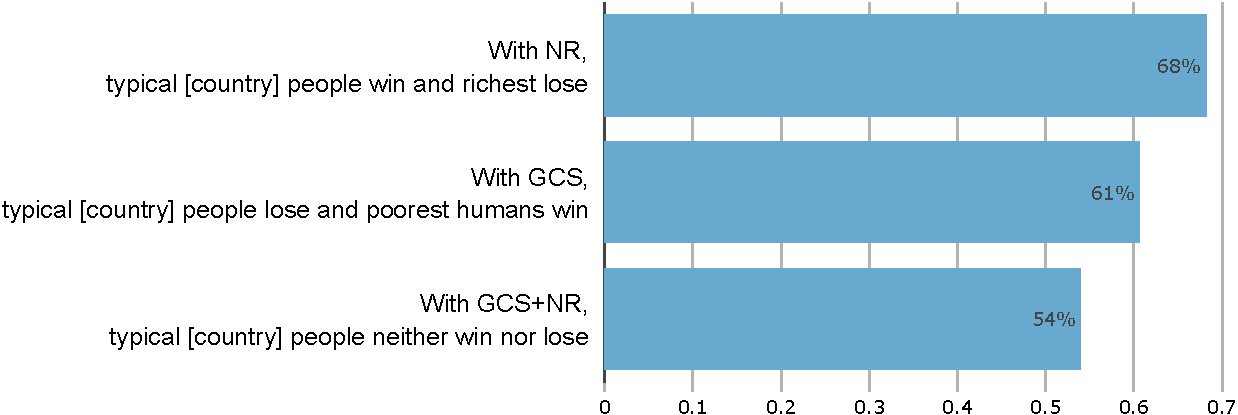
\includegraphics[width=\textwidth]{../figures/US1/understood_each.pdf}} 
\end{figure}

\begin{figure}[h!]
    \caption[Comprehension score]{Number of correct answers to comprehension questions (mean). (Questions \ref{q:understood_gcs}-\ref{q:understood_both})}\label{fig:understood_score}
    \makebox[\textwidth][c]{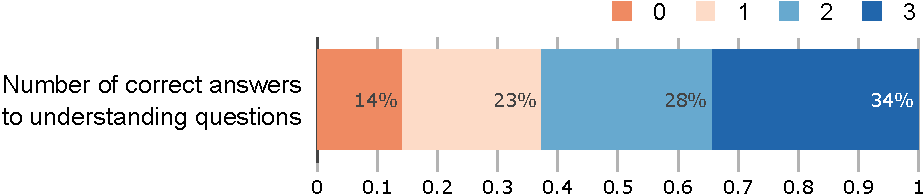
\includegraphics[width=\textwidth]{../figures/US1/understood_score.pdf}} 
\end{figure}

\begin{figure}[h!]
    \caption[Support for the GCS]{Support for the GCS, NR and the combination of GCS, NR and C. (Questions \ref{q:gcs_support}, \ref{q:nr_support} and \ref{q:crg_support})}\label{fig:support_binary}
    \makebox[\textwidth][c]{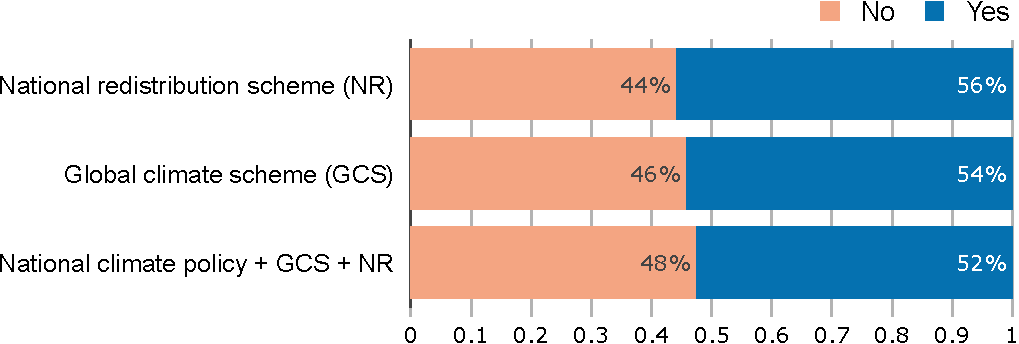
\includegraphics[width=.9\textwidth]{../figures/US1/support_binary.pdf}} 
\end{figure}

\begin{figure}[h!]
    \caption[Beliefs about support for the GCS and NR]{Beliefs regarding the support for the GCS and NR. (Questions \ref{q:gcs_belief} and \ref{q:nr_belief})}\label{fig:belief}
    \makebox[\textwidth][c]{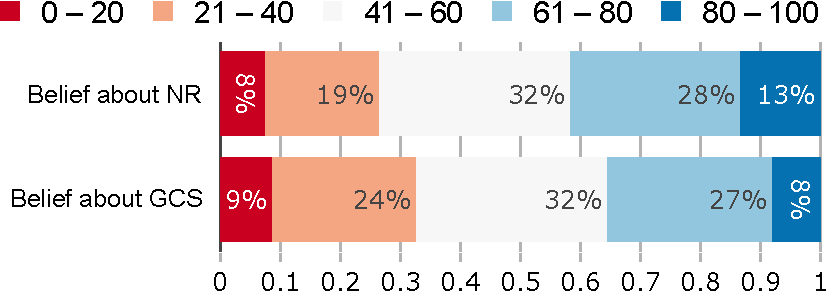
\includegraphics[width=.8\textwidth]{../figures/US1/belief.pdf}} 
\end{figure}

\begin{figure}[h!]
    \caption[List experiment]{List experiment: mean number of supported policies. ( Question \ref{q:list_exp})}\label{fig:list_exp}
    \makebox[\textwidth][c]{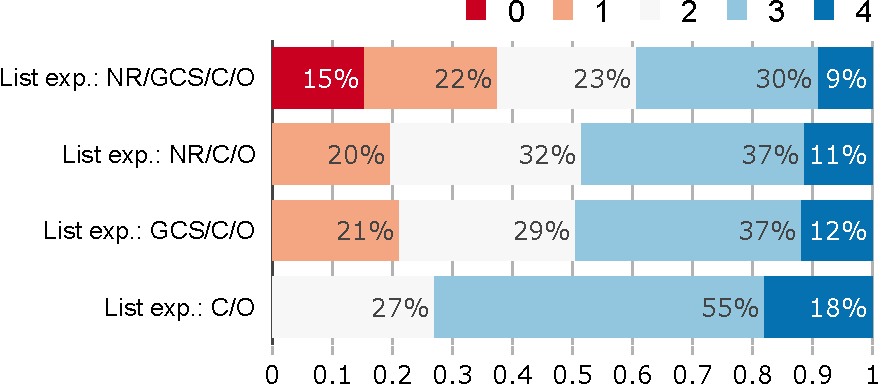
\includegraphics[width=.8\textwidth]{../figures/US1/list_exp.pdf}} 
\end{figure}

\begin{figure}[h!]
    \caption[Conjoint analyses]{Conjoint analyses. (Questions \ref{q:conjoint_a}-\ref{q:conjoint_d})}\label{fig:conjoint}
    \makebox[\textwidth][c]{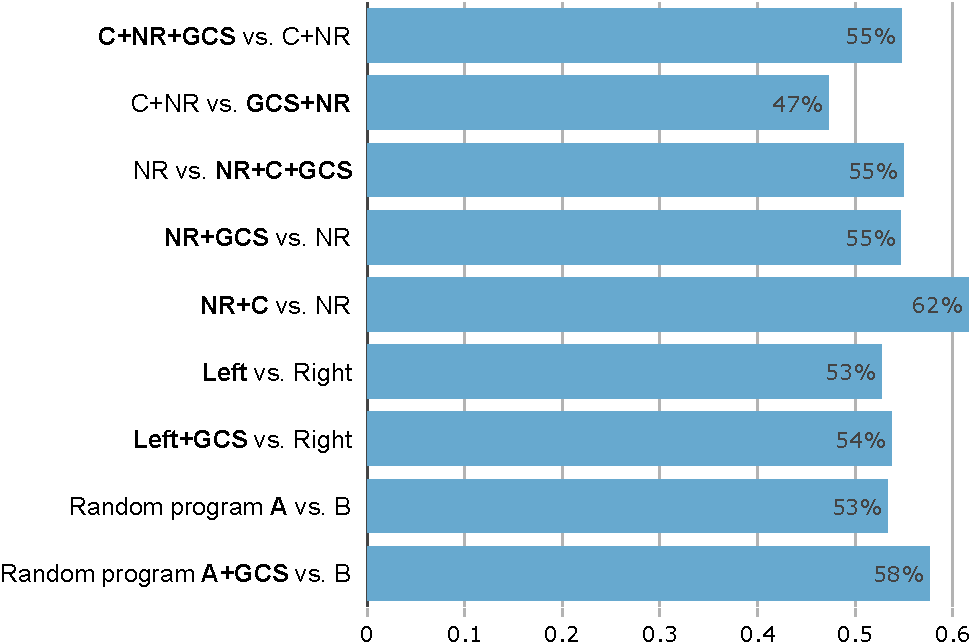
\includegraphics[width=\textwidth]{../figures/US1/conjoint.pdf}} 
\end{figure}

\begin{figure}[h!] 
    \caption[Preferences for various policies in Democratic platforms]{Effects of the presence of a policy (rather than none from this domain) in a random Democratic platform on the likelihood that it is preferred to another random Democratic platform. [Asked only to non-Republicans] (Question \ref{q:conjoint_r}%; in the U.S., asked only to non-Republicans.
    )}\label{fig:ca_r}
    \makebox[\textwidth][c]{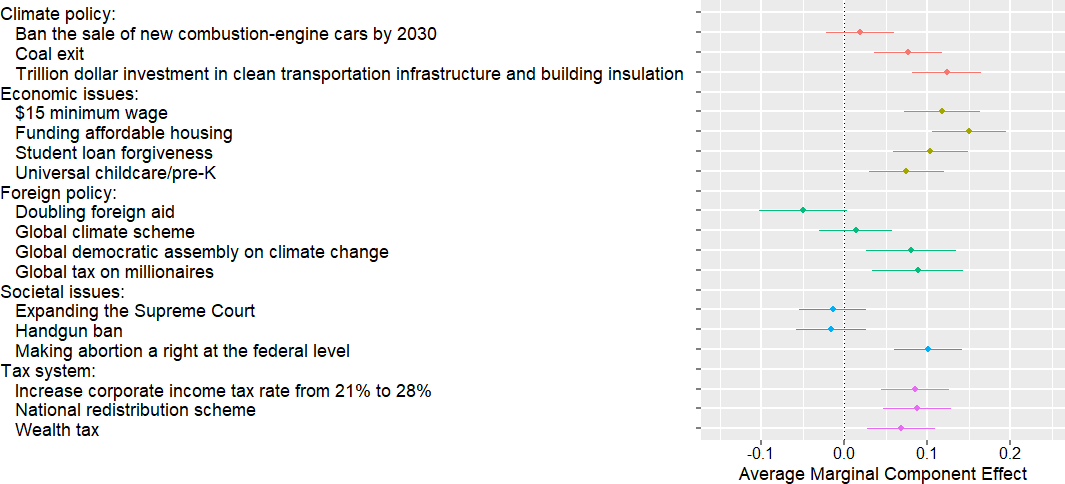
\includegraphics[width=\textwidth]{../figures/US1/ca_r.png}} 
\end{figure}

\begin{figure}[h!] % TODO: US2
    \caption[Perceptions of the GCS]{Perceptions of the GCS. Importance of elements for supporting the GCS (in percent). (Question \ref{q:gcs_important})}\label{fig:gcs_important}
    \makebox[\textwidth][c]{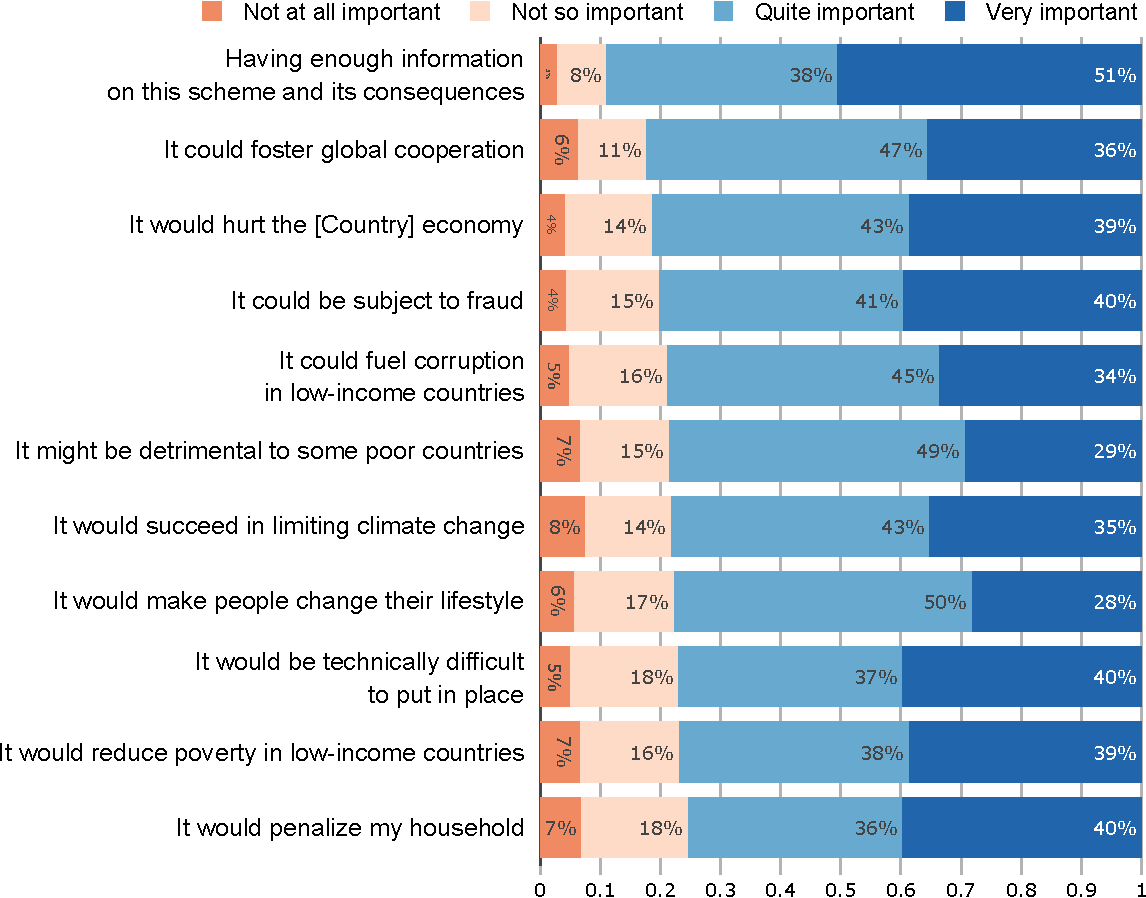
\includegraphics[width=\textwidth]{../figures/US2/gcs_important.pdf}} 
\end{figure}

\begin{figure}[h!]
    \caption[Donation to Africa vs. own country]{Donation in case of lottery win, depending on the recipient's (randomly drawn) nationality (mean). (Question \ref{q:donation})}\label{fig:donation}
    \makebox[\textwidth][c]{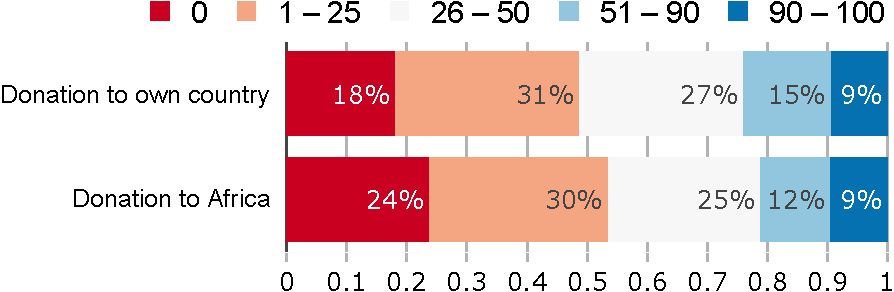
\includegraphics[width=.8\textwidth]{../figures/US1/variables_donation.pdf}} 
\end{figure}

\begin{figure}[h!] % TODO: US2
    \caption[Support for various global policies]{Support for various global policies. (Questions \ref{q:climate_policies}, \ref{q:other_policies}, \ref{q:global_tax} and \ref{q:national_tax})}\label{fig:support_likert}\label{fig:support}
    \makebox[\textwidth][c]{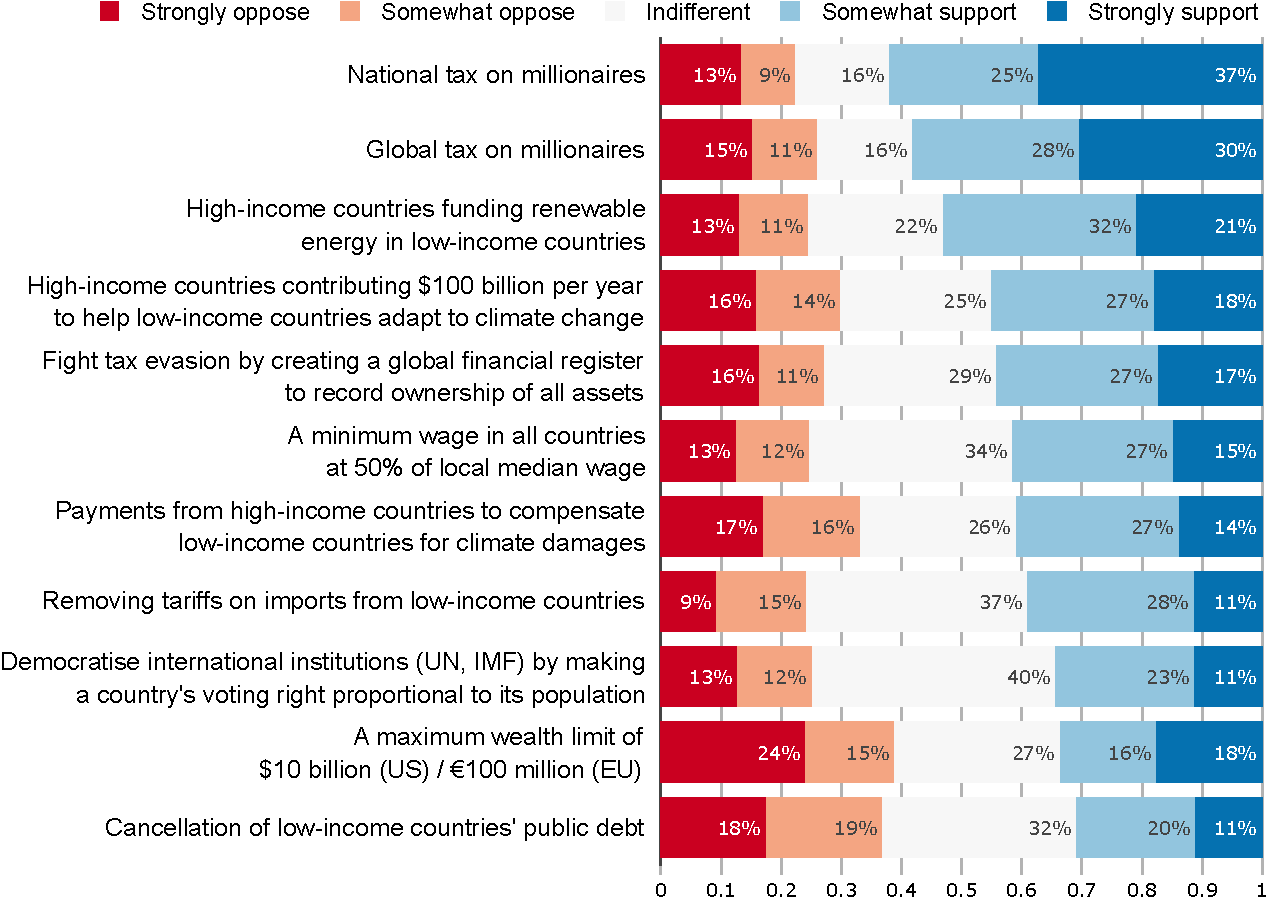
\includegraphics[width=\textwidth]{../figures/US/support_likert.pdf}} 
\end{figure}

% \begin{figure}[h!]
%     \caption{label}\label{fig:climate_policies}
%     \makebox[\textwidth][c]{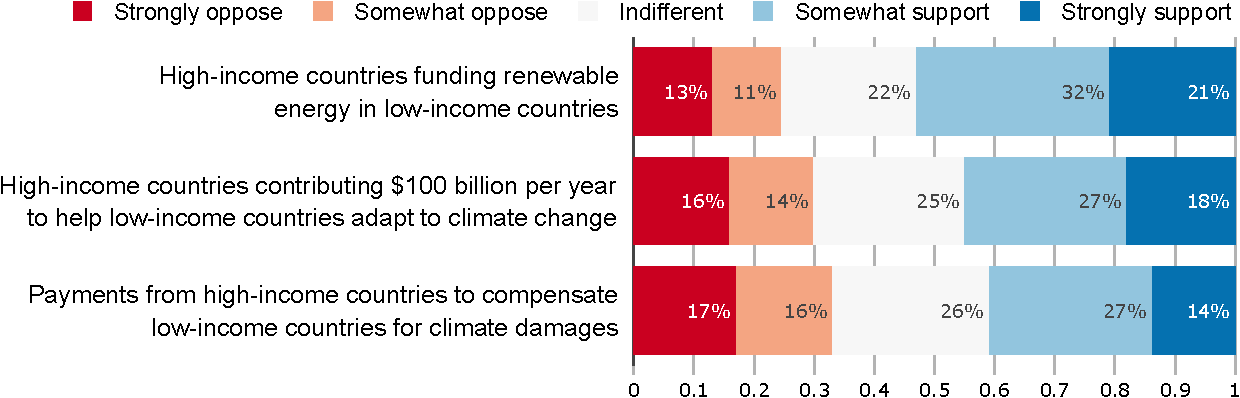
\includegraphics[width=\textwidth]{../figures/US1/climate_policies.pdf}} 
% \end{figure}

% \begin{figure}[h!]
%     \caption{label}\label{fig:global_policies}
%     \makebox[\textwidth][c]{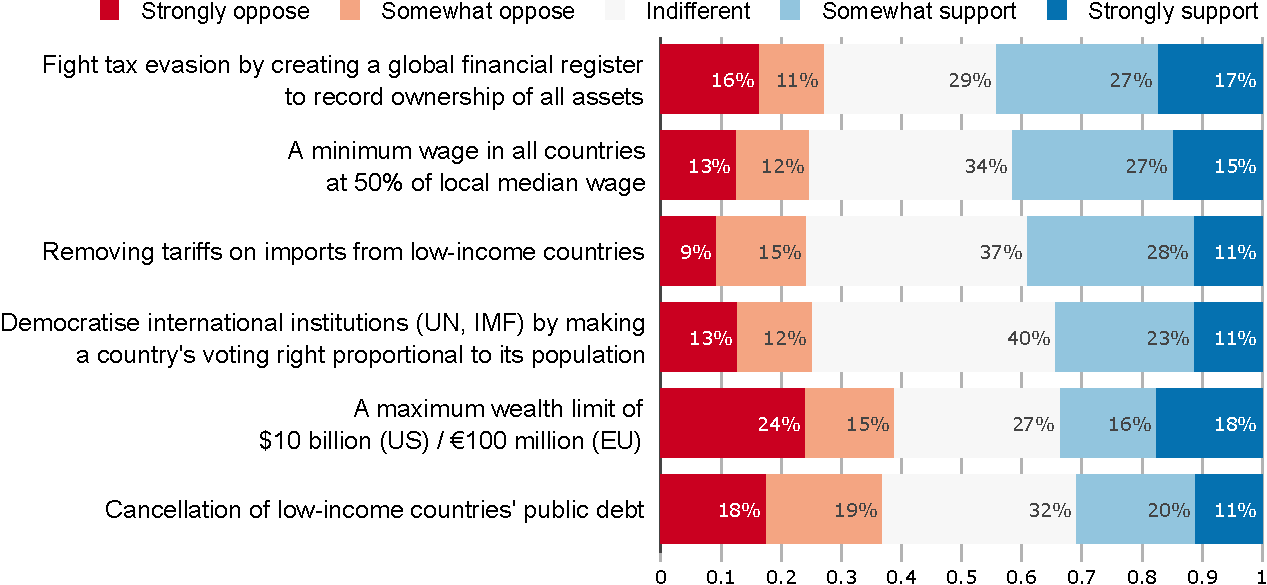
\includegraphics[width=\textwidth]{../figures/US1/global_policies.pdf}} 
% \end{figure}

\begin{figure}[h!] % TODO: US2
    \caption[Preferred share of global tax for low-income countries]{Preferred share of global wealth tax revenues that should be pooled to finance low-income countries. (Question \ref{q:global_tax_global_share})}\label{fig:global_tax_global_share}
    \makebox[\textwidth][c]{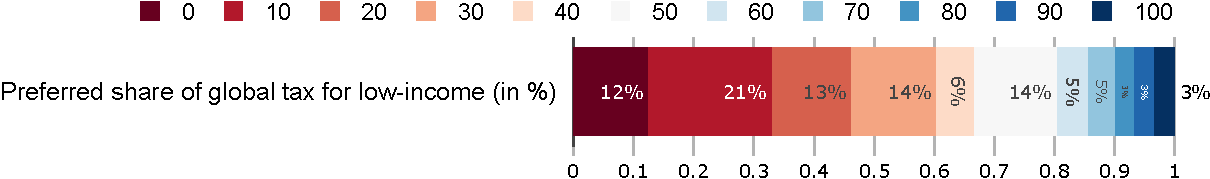
\includegraphics[width=\textwidth]{../figures/US2/global_tax_global_share.pdf}} 
\end{figure}

\begin{figure}[h!] % TODO: US2
    \caption[Preferred share of global tax for low-income countries (summary)]{Prefences on the share of global wealth tax revenues that should be pooled to finance low-income countries. (Questions \ref{q:global_tax_global_share} and \ref{q:global_tax_sharing})}\label{fig:global_tax_share}\label{fig:global_tax_sharing}
    \makebox[\textwidth][c]{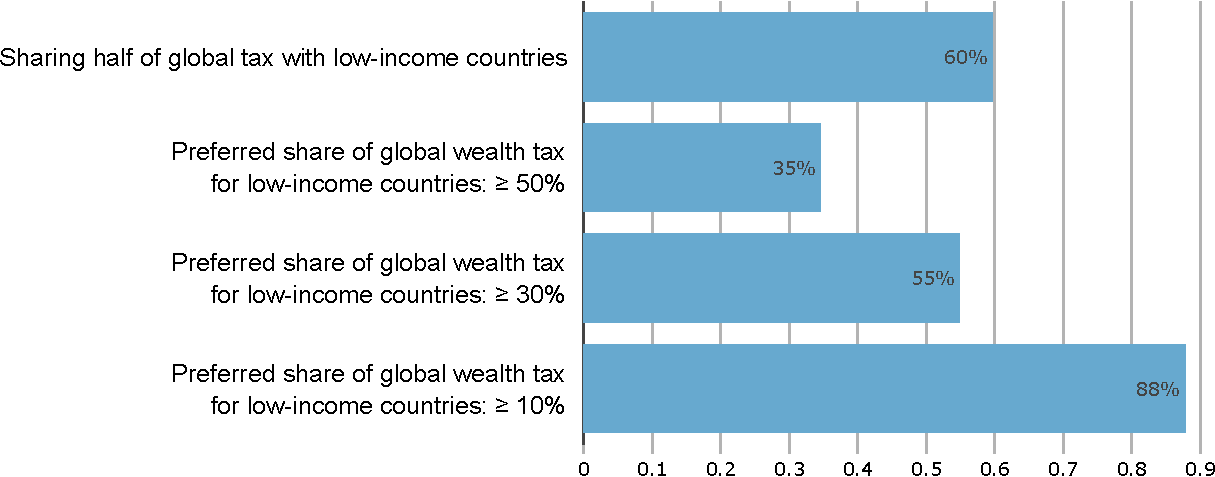
\includegraphics[width=\textwidth]{../figures/US2/global_tax_share.pdf}} 
\end{figure}

\begin{figure}[h!] % TODO: US2
    \caption[Perceived and preferred foreign aid]{Perceived and preferred foreign aid (with or without information on actual amount). (Questions \ref{q:foreign_aid_belief} and \ref{q:foreign_aid_preferred})}\label{fig:foreign_aid_belief}\label{fig:foreign_aid_preferred_no_info}\label{fig:foreign_aid_preferred_info}\label{fig:foreign_aid_amount}
    \makebox[\textwidth][c]{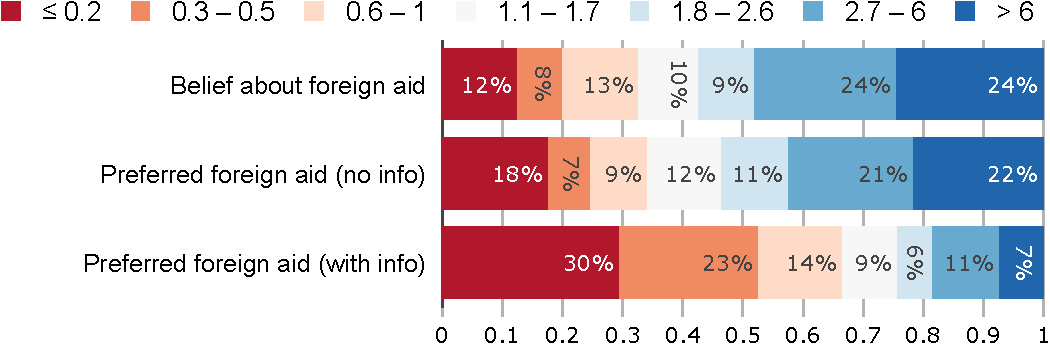
\includegraphics[width=\textwidth]{../figures/US2/foreign_aid_amount.pdf}} 
\end{figure}

\begin{figure}[h!] % TODO: US2
    \caption[Preferences for funding increased foreign aid]{Preferences for funding increased foreign aid. [Asked iff preferred foreign aid is strictly greater than [Info: actual; No info: perceived] foreign aid] \\ ``How would you like to finance such increase in foreign aid? (Multiple answers possible)'' (in percent) (Question \ref{q:foreign_aid_raise_how})}\label{fig:foreign_aid_raise_how}
    \makebox[\textwidth][c]{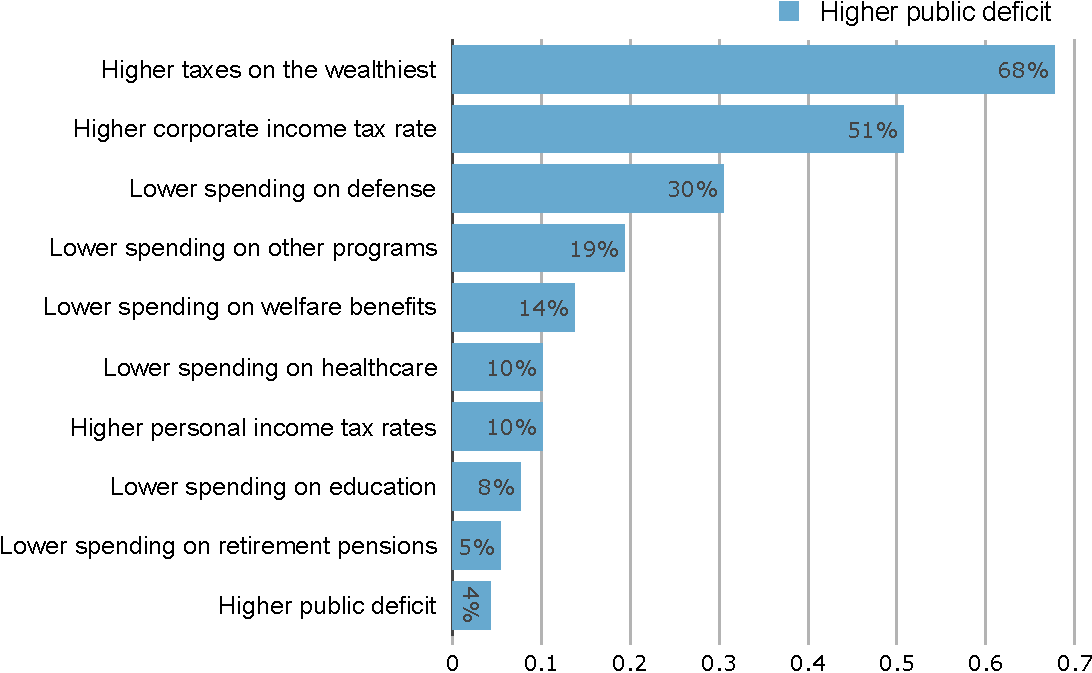
\includegraphics[width=.75\textwidth]{../figures/US2/foreign_aid_raise.pdf}} 
\end{figure}

\begin{figure}[h!] % TODO: US2
    \caption[Preferences of spending following reduced foreign aid]{Preferences of spending following reduced foreign aid. [Asked iff preferred foreign aid is strictly lower than [Info: actual; No info: perceived] foreign aid] \\ ``How would you like to use the freed budget? (Multiple answers possible)'' (in percent) (Question \ref{q:foreign_aid_reduce_how})}\label{fig:foreign_aid_reduce_how}
    \makebox[\textwidth][c]{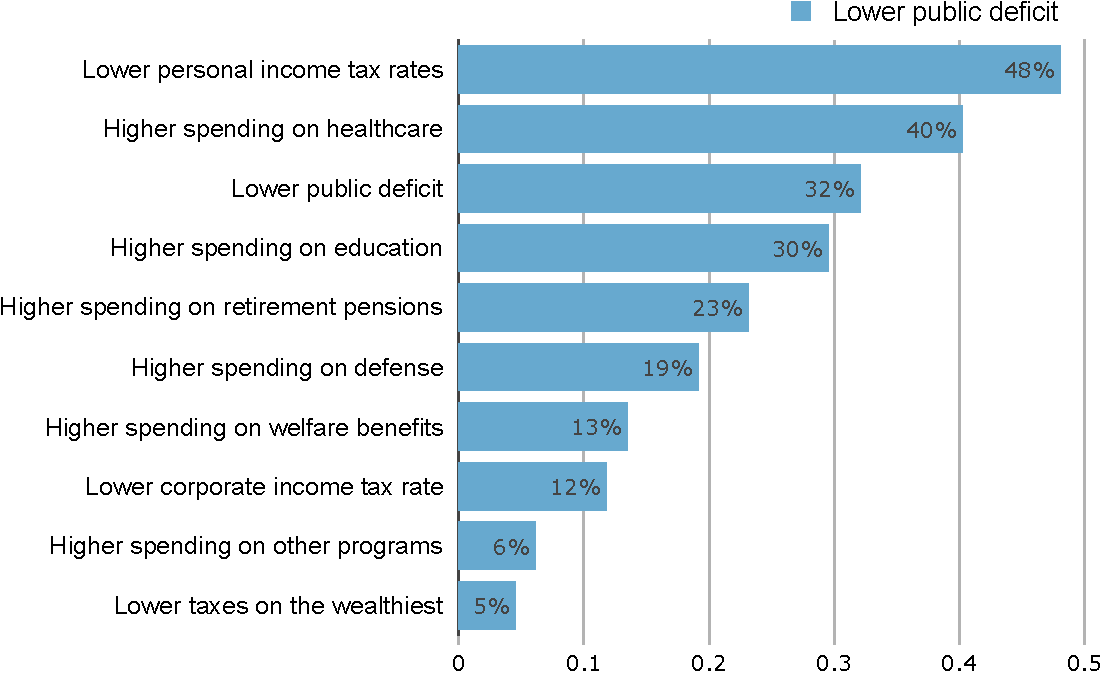
\includegraphics[width=.75\textwidth]{../figures/US2/foreign_aid_reduce.pdf}} 
\end{figure}

\begin{figure}[h!]
    \caption[Attitudes on the evolution of foreign aid]{Attitudes regarding the evolution of U.S. foreign aid. (Question \ref{q:foreign_aid_raise_support})}\label{fig:foreign_aid_raise_support}
    \makebox[\textwidth][c]{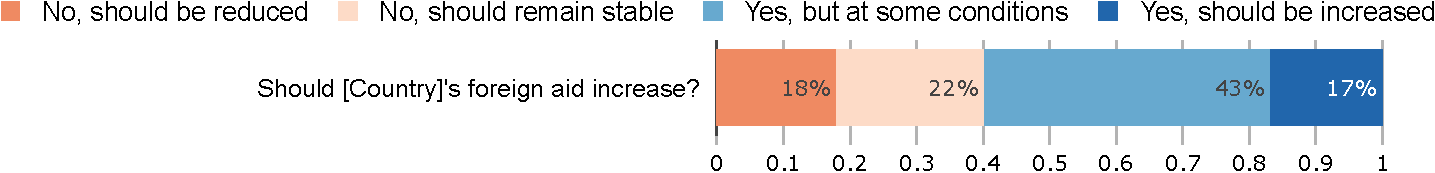
\includegraphics[width=\textwidth]{../figures/US1/foreign_aid_raise_support.pdf}} 
\end{figure}

\begin{figure}[h!]
    \caption[Conditions at which foreign aid should be increased]{Conditions at which foreign aid should be increased (in percent). [Asked to those who wish an increase of foreign aid at some conditions.] (Question \ref{q:foreign_aid_condition})}\label{fig:foreign_aid_condition}
    \makebox[\textwidth][c]{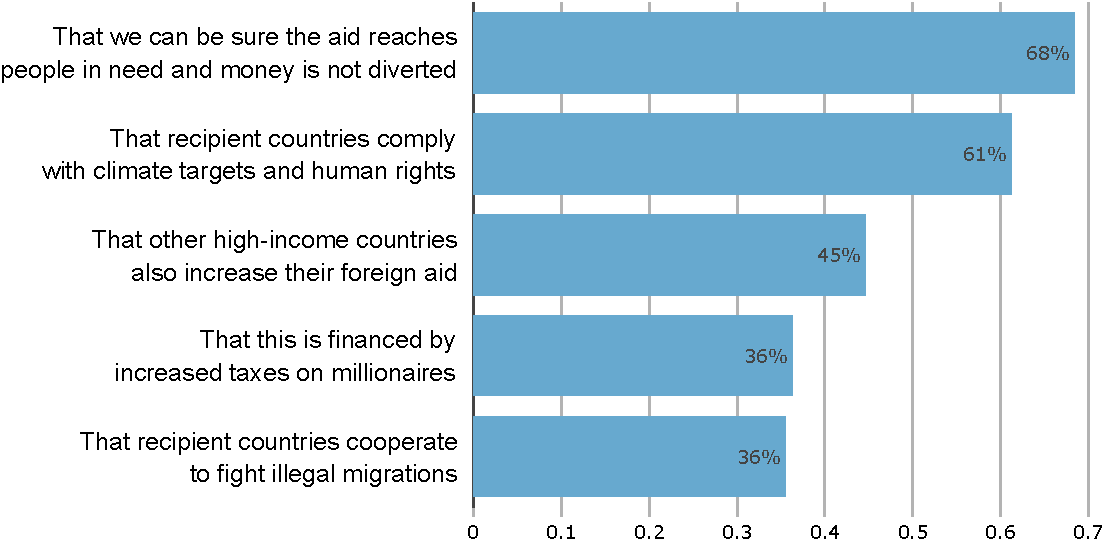
\includegraphics[width=\textwidth]{../figures/US1/foreign_aid_condition.pdf}} 
\end{figure}

\begin{figure}[h!]
    \caption[Reasons why foreign aid should not be increased]{Reasons why foreign aid should not be increased (in percent). [Asked to those who wish a decrease or stability of foreign aid.] (Question \ref{q:foreign_aid_no})}\label{fig:foreign_aid_no}
    \makebox[\textwidth][c]{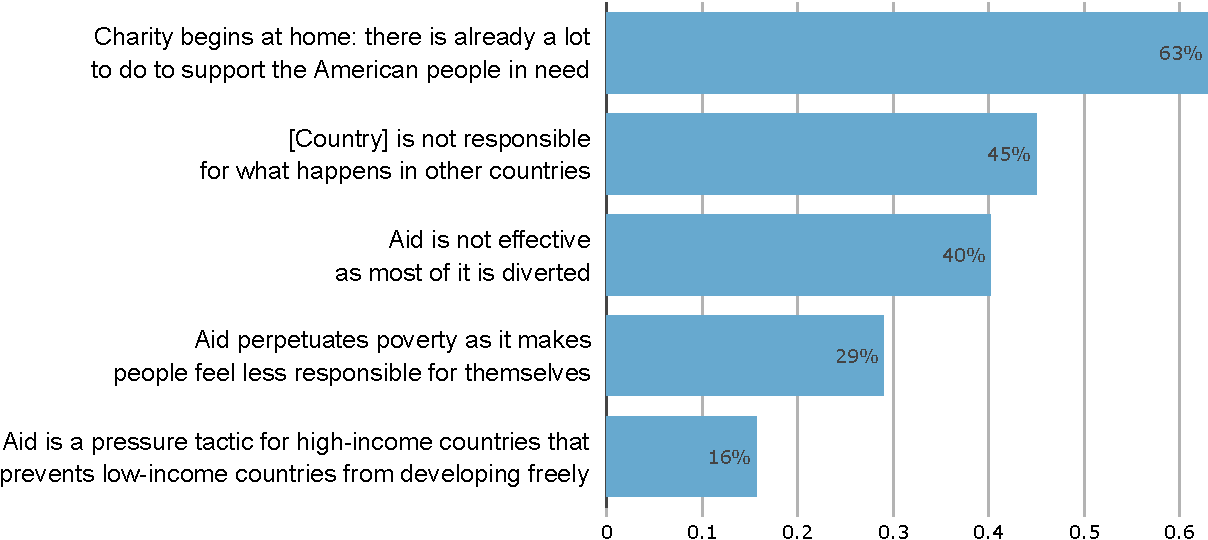
\includegraphics[width=\textwidth]{../figures/US1/foreign_aid_no.pdf}} 
\end{figure}

\begin{figure}[h!]
    \caption[Willingness to sign a real-stake petition]{Willingness to sign real-stake petition for the Global Climate Scheme or National Redistribution. (Question \ref{q:petition})}\label{fig:petition}
    \makebox[\textwidth][c]{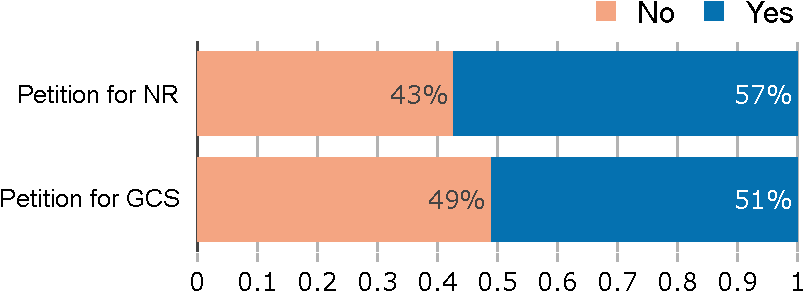
\includegraphics[width=.7\textwidth]{../figures/US1/variables_petition.pdf}} 
\end{figure}

\begin{figure}[h!]
    \caption[Preferred approach for international climate negotiations]{Preferred approach of diplomats at international climate negotiations. \\ In international climate negotiations, would you prefer U.S. diplomats to defend U.S. interests or global justice? (Question \ref{q:negotiation})}\label{fig:negotiation}
    \makebox[\textwidth][c]{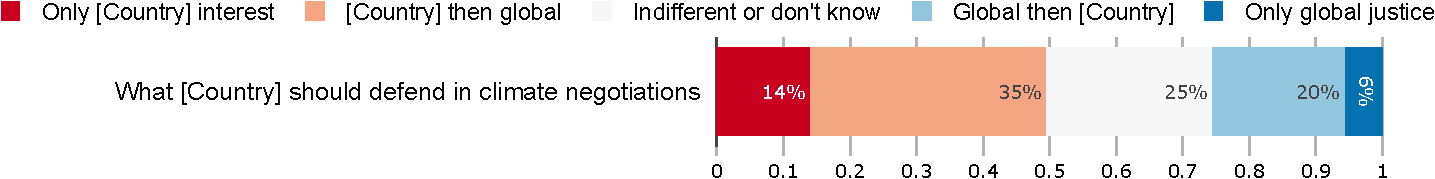
\includegraphics[width=\textwidth]{../figures/US1/negotiation.pdf}} 
\end{figure}

\begin{figure}[h!]
    \caption[Importance of selected issues]{Importance of selected issues.\\ ``To what extent do you think the following issues are a problem?'' (Question \ref{q:problem})}\label{fig:problem}
    \makebox[\textwidth][c]{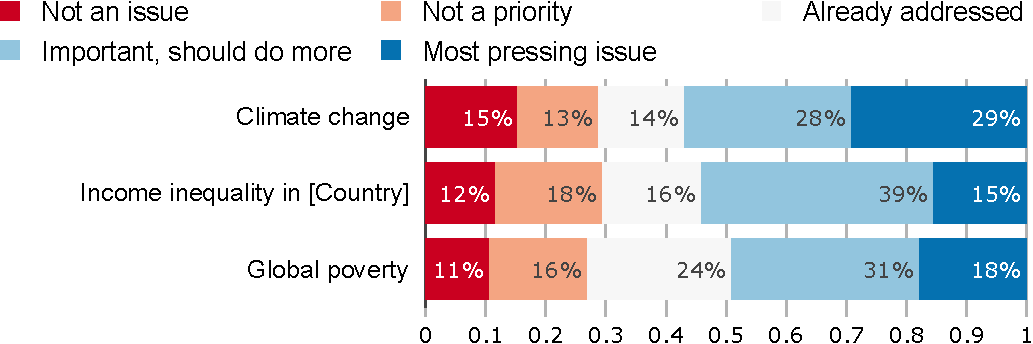
\includegraphics[width=\textwidth]{../figures/US1/problem.pdf}} 
\end{figure}

\begin{figure}[h!]
    \caption[Group defended when voting (aggregated)]{Group defended when voting (aggregated). \\ ``What group do you defend when you vote?'' (Question \ref{q:group_defended})}\label{fig:group_defended}
    \makebox[\textwidth][c]{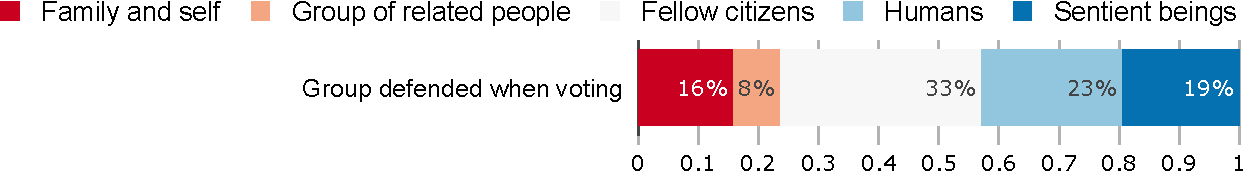
\includegraphics[width=\textwidth]{../figures/US1/group_defended_agg2.pdf}} 
\end{figure}

\begin{figure}[h!]
    \caption[Group defended when voting]{Group defended when voting. \\ ``What group do you defend when you vote?'' (Question \ref{q:group_defended})}\label{fig:group_defended}
    \makebox[\textwidth][c]{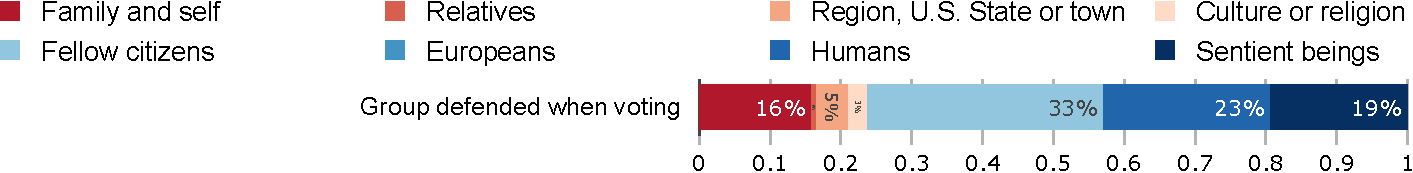
\includegraphics[width=\textwidth]{../figures/US1/group_defended.pdf}} 
\end{figure}

\begin{figure}[h!] % already in text
    \caption[Prioritization of policies]{Prioritization of policies. \\Number of points allocated policies to express intensity of support (among six policies chosen at random). (Question \ref{q:points})}\label{fig:points}
    \makebox[\textwidth][c]{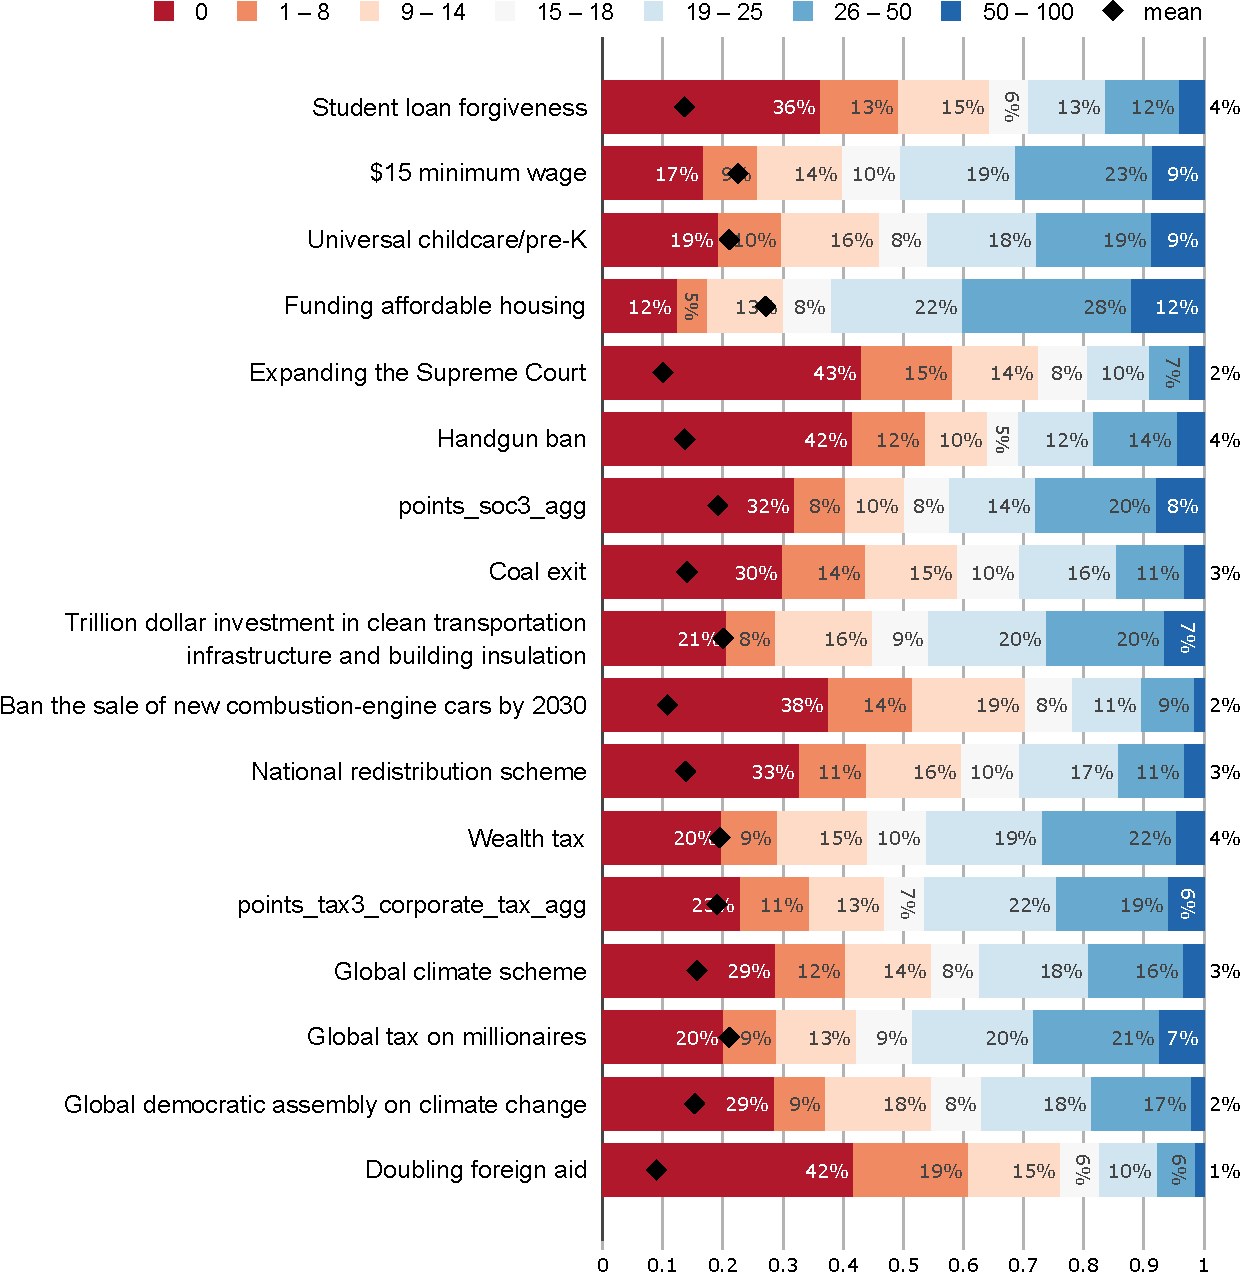
\includegraphics[width=\textwidth]{../figures/US1/points_mean.pdf}} 
\end{figure}

\begin{figure}[h!] % TODO: US
    \caption[Charity donation]{Charity donation. \\ ``How much did you give to charities in 2022?'' (Question \ref{q:donation_charities})}\label{fig:donation_charities}
    \makebox[\textwidth][c]{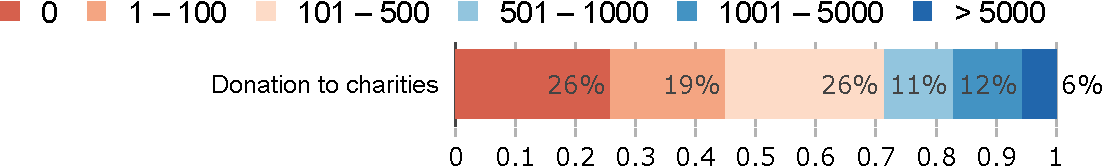
\includegraphics[width=.8\textwidth]{../figures/US/donation_charities.pdf}} 
\end{figure}

% \begin{figure}[h!] 
%     \caption[Interest in politics]{Interest in politics. \\ ``To what extent are you interested in politics?'' (Question \ref{q:interested_politics})}\label{fig:interested_politics}
%     \makebox[\textwidth][c]{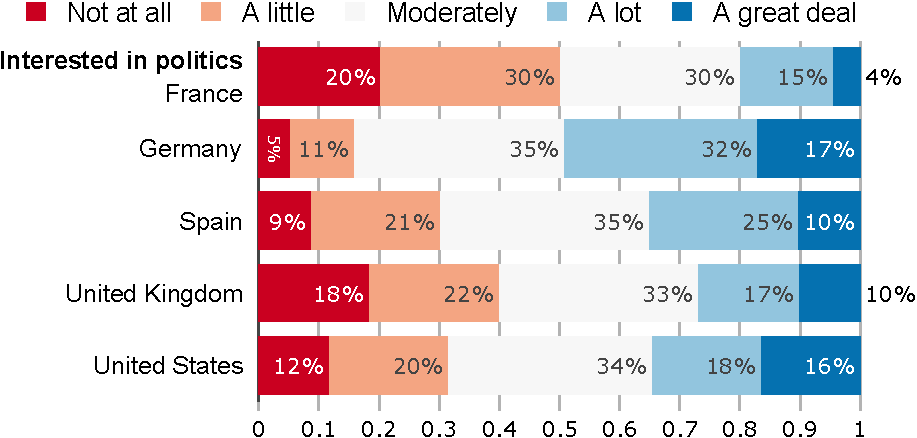
\includegraphics[width=.8\textwidth]{../figures/country_comparison/interested_politics.pdf}} 
% \end{figure}

% \begin{figure}[h!] 
%     \caption[Desired involvement of government]{Desired involvement of government (from 1 to 5). (Question \ref{q:involvement_govt})}\label{fig:involvement_govt}
%     \makebox[\textwidth][c]{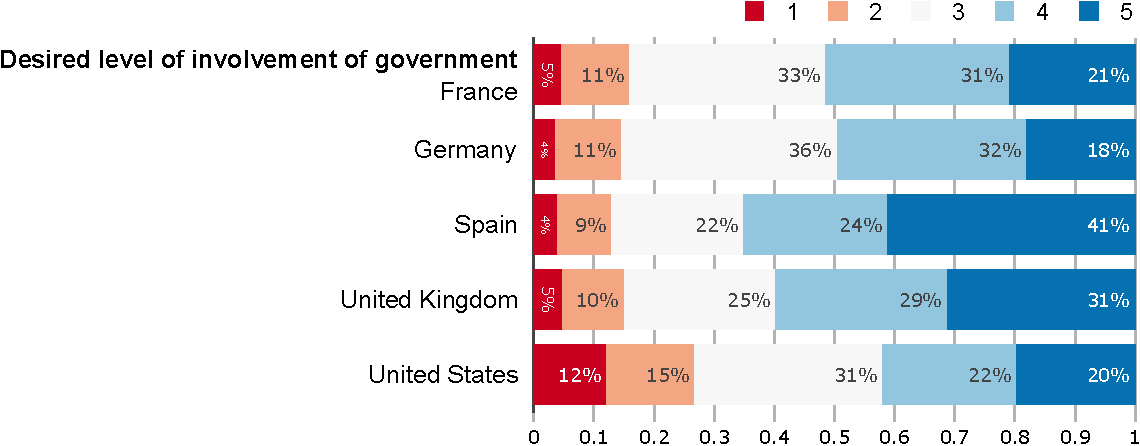
\includegraphics[width=.9\textwidth]{../figures/country_comparison/involvement_govt.pdf}} 
% \end{figure}

% \begin{figure}[h!] 
%     \caption[Political leaning]{Political leaning on economics (from 1: Left to 5: Right). (Question \ref{q:left_right})}\label{fig:left_right}
%     \makebox[\textwidth][c]{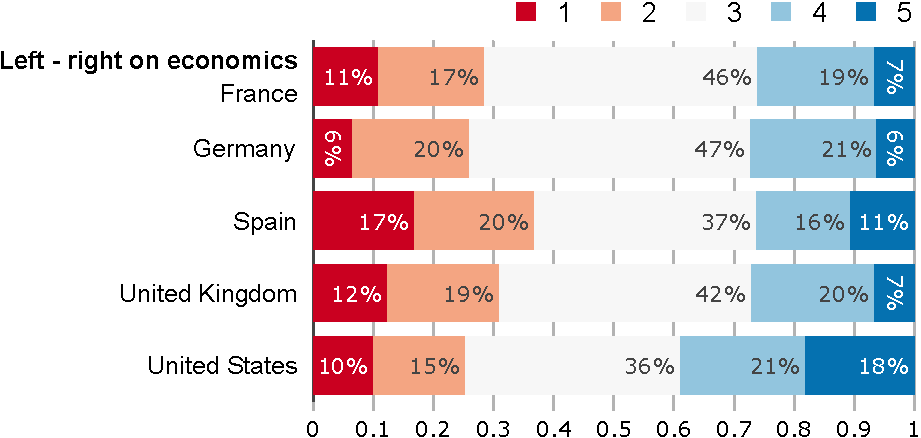
\includegraphics[width=.8\textwidth]{../figures/country_comparison/left_right.pdf}} 
% \end{figure}

\begin{figure}[h!]  % TODO: Eu
    \caption[Political affiliation (US1)]{Political affiliation (US1). (Question \ref{q:political_affiliation})}\label{fig:political_affiliation}
    \makebox[\textwidth][c]{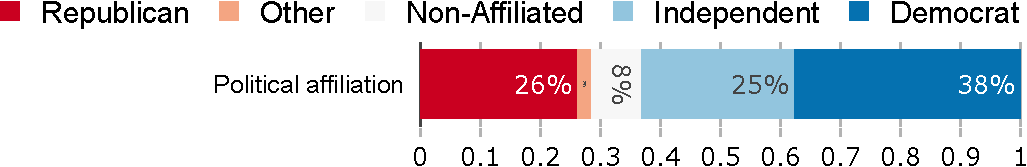
\includegraphics[width=.8\textwidth]{../figures/US1/political_affiliation.pdf}} 
\end{figure}

\begin{figure}[h!] 
    \caption[Political affiliation (US2)]{Political affiliation (US2). (Question \ref{q:political_affiliation})}\label{fig:political_affiliation}
    \makebox[\textwidth][c]{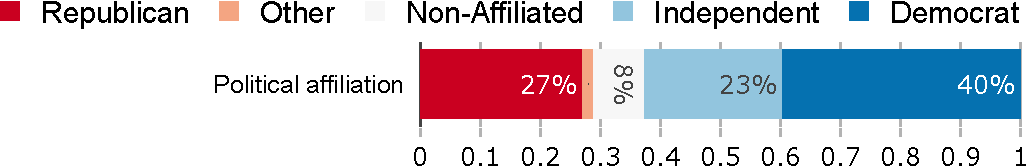
\includegraphics[width=.8\textwidth]{../figures/US2/political_affiliation.pdf}} 
\end{figure} % TODO: have only one figure with two lines: US1 and US2

\begin{figure}[h!] 
    \caption[Voted in last election (US1)]{Voted in last election (US1). (Question \ref{q:vote_participation})}\label{fig:vote_participation}
    \makebox[\textwidth][c]{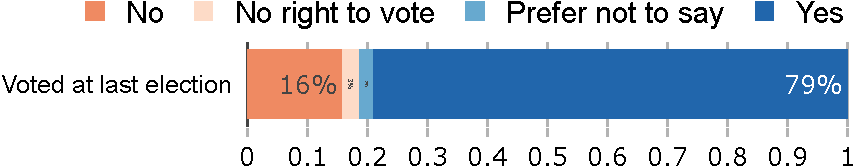
\includegraphics[width=.8\textwidth]{../figures/US1/vote_participation.pdf}} 
\end{figure}

\begin{figure}[h!] 
    \caption[Voted in last election (US2)]{Voted in last election (US2). (Question \ref{q:vote_participation})}\label{fig:vote_participation}
    \makebox[\textwidth][c]{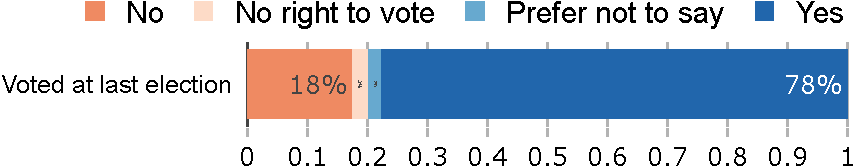
\includegraphics[width=.8\textwidth]{../figures/US2/vote_participation.pdf}} 
\end{figure}

\begin{figure}[h!]
    \caption[Vote in last election (US1)]{Vote in last election (US2). (Question \ref{q:vote})}\label{fig:vote}
    \makebox[\textwidth][c]{\includegraphics[width=.75\textwidth]{../figures/US1/vote_us_comp.pdf}} 
\end{figure}

\begin{figure}[h!]
    \caption[Vote in last election (US2)]{Vote in last election (US2). (Question \ref{q:vote})}\label{fig:vote}
    \makebox[\textwidth][c]{\includegraphics[width=.75\textwidth]{../figures/US2/vote_us_comp.pdf}} 
\end{figure}

\begin{figure}[h!] % TODO: Eu replace by vote_agg
    \caption[Actual or hypothetical vote in last election (US1)]{Actual or hypothetical vote in last election (US1). (Question \ref{q:vote})}\label{fig:vote}
    \makebox[\textwidth][c]{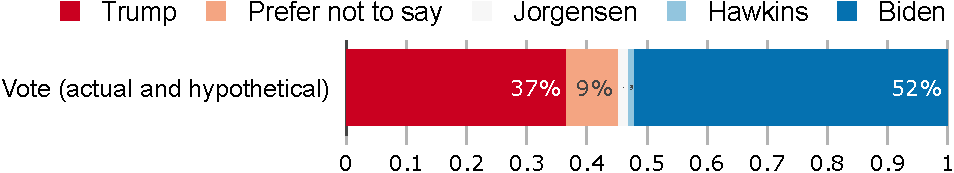
\includegraphics[width=.75\textwidth]{../figures/US1/vote_all.pdf}} 
\end{figure}

\begin{figure}[h!] 
    \caption[Actual or hypothetical vote in last election (US2)]{Actual or hypothetical vote in last election (US2). (Question \ref{q:vote})}\label{fig:vote}
    \makebox[\textwidth][c]{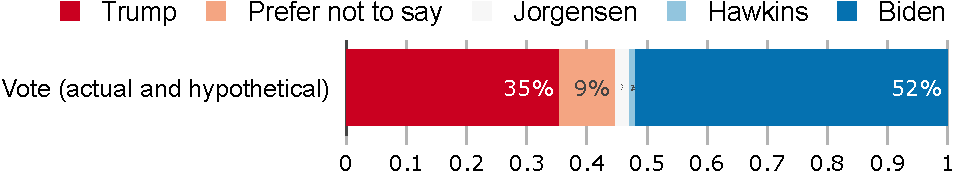
\includegraphics[width=.75\textwidth]{../figures/US2/vote_all.pdf}} 
\end{figure}

\begin{figure}[h!] 
    \caption[Perception that survey was biased (US1)]{Perception that survey was biased (US1). \\ ``Do you feel that this survey was politically biased?'' (Question \ref{q:survey_biased})}\label{fig:survey_biased}
    \makebox[\textwidth][c]{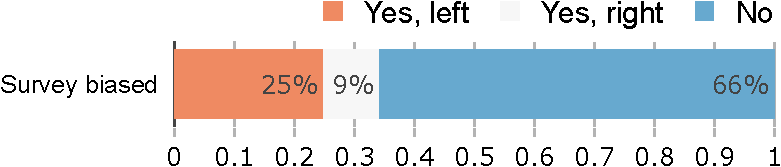
\includegraphics[width=.7\textwidth]{../figures/US1/survey_biased.pdf}} 
\end{figure}

\begin{figure}[h!] TODO US2
    \caption[Perception that survey was biased (US2)]{Perception that survey was biased (US2). \\ ``Do you feel that this survey was politically biased?'' (Question \ref{q:survey_biased})}\label{fig:survey_biased}
    \makebox[\textwidth][c]{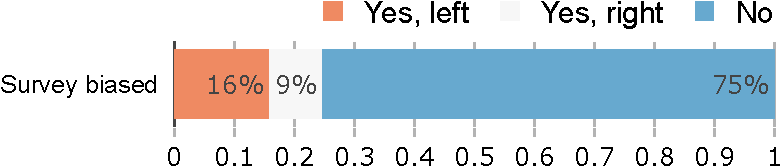
\includegraphics[width=.7\textwidth]{../figures/US2/survey_biased.pdf}} 
\end{figure}

% \begin{figure}[h!] 
%     \caption[Interested to be interviewed]{Interested to be interviewed by a researcher for 30 min through videoconference. (Question \ref{q:interview})}\label{fig:interview}
%     \makebox[\textwidth][c]{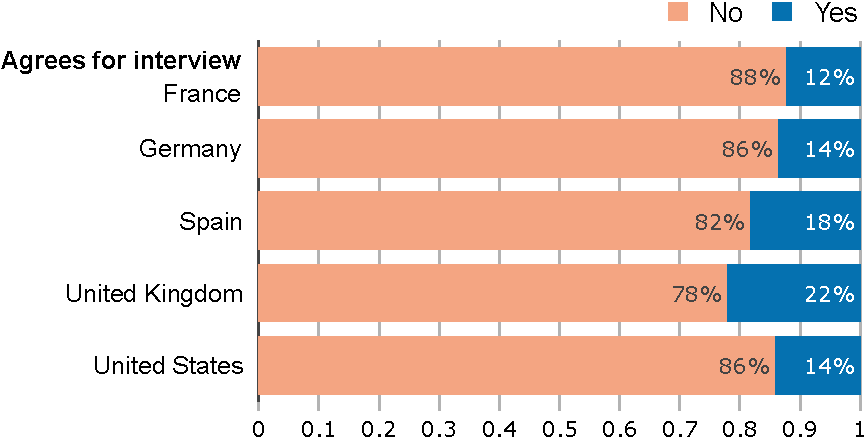
\includegraphics[width=\textwidth]{../figures/country_comparison/interview.pdf}} 
% \end{figure}   

% \begin{figure}[h!]
%     \caption{label}\label{fig:share_policies_supported}
%     \makebox[\textwidth][c]{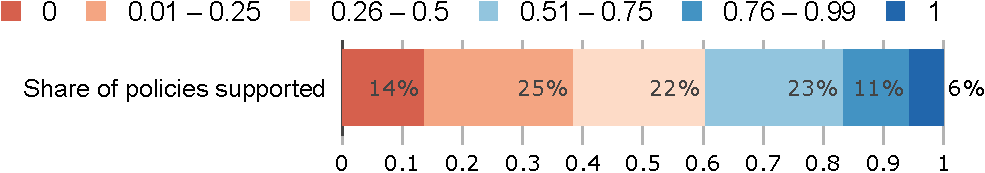
\includegraphics[width=\textwidth]{../figures/US1/share_policies_supported.pdf}} 
% \end{figure} % TODO? uncomment?

% \begin{figure}[h!]
%     \caption{label}\label{fig:vars}
%     \makebox[\textwidth][c]{\includegraphics[width=\textwidth]{../figures/US1/vars.pdf}} 
% \end{figure}

\clearpage
\section{Questionnaire}
\input{app_questionnaire} % TODO: use specific rather than generic questionnaire

\end{document}
